%% LyX 2.3.7 created this file.  For more info, see http://www.lyx.org/.
%% Do not edit unless you really know what you are doing.
\documentclass[english]{article}
\usepackage[T1]{fontenc}
\usepackage[latin9]{inputenc}
\usepackage{float}
\usepackage{url}

\makeatletter
%%%%%%%%%%%%%%%%%%%%%%%%%%%%%% User specified LaTeX commands.
\usepackage{graphics}
\usepackage{subcaption}

\makeatother

\usepackage{babel}
\begin{document}
\title{OPTIMUS: a multidimensional global optimization package}
\author{$ $}
\date{$ $}
\maketitle
\begin{abstract}
A significant number of applications from many research areas can
be considered global optimization problems, such as applications in
the area of image processing, medical informatics, economic models,
etc. This paper presents a programming tool written in ANSI C++, which
researchers can use to formulate the problem to be solved and then
make use of the local and global optimization methods provided by
this tool to efficiently solve such problems. The main features of
the suggested software are: a) Coding of the objective problem in
a high level language such as ANSI C++ b) Incorporation of many global
optimization techniques to tackle the objective problem c)Parameterization
of global optimization methods using user-defined parameters d) Usage
of a GUI application to control the optimization strategy.
\end{abstract}

\section{Introduction}

The location of the global minimum for a continuous and differentiable
function $f:S\rightarrow R,S\subset R^{n}$ is formulated as
\begin{equation}
x^{*}=\mbox{arg}\min_{x\in S}f(x)\label{eq:eq1}
\end{equation}
where the set $S$ is defined as: 
\[
S=\left[a_{1},b_{1}\right]\otimes\left[a_{2},b_{2}\right]\otimes\ldots\left[a_{n},b_{n}\right]
\]
Methods that aim to locate the global minimum finds application in
problems from the area of economics \cite{globalecon1,globalecon2},
problems that appear very often in the area of physics \cite{global_physics1,global_physics2},
chemistry \cite{global_chemistry1,global_chemistry2}, common problems
from medicine \cite{global_med1,global_med2}, job scheduling problems
\cite{global_job1,global_job2}, water resources planning \cite{global_water1,global_water2},
network security problems \cite{global_network1,global_network2},
robotics \cite{global_robot1,global_robot2} etc. Also, global optimization
methods were used on some symmetry problems \cite{go_symmetry0,go_symmetry1,go_symmetry2}
as well as on inverse problems \cite{global_nonlinear1,global_nonlinear2,global_nonlinear3}.
In the relevant literature there are a number of global optimization
techniques, such as Adaptive Random Search methods \cite{go_adaptive1,go_adaptive2},
Controlled Random Search methods \cite{go_crs1,go_crs2}, Simulated
Annealing \cite{go_sa1,go_sa2,go_sa3}, Genetic algorithms \cite{go_ga1,go_ga2},
Ant Colony Optimization \cite{go_ant1,go_ant2}, Particle Swarm Optimization
\cite{go_pso1,go_pso2} etc. 

Due to the high importance of the global optimization problem, a variety
of hybrid optimization techniques have been proposed to handle the
global optimization problem, such as methods that combine Particle
Swarm Optimization and Genetic algorithms \cite{go_pso_genetic_hybrid1,go_pso_genetic_hybrid2},
combination of genetic algorithms and fuzzy logic classifier \cite{ga_fuzzy},
incorporation of genetic algorithm and the K-Means algorithm \cite{ga_kmeans},
combination of Particle Swarm Optimization method with Ant Colony
Optimization \cite{pso_aco1,pso_aco2,pso_aco3}, methods that combine
the Simplex method and Inductive search \cite{hybrid1} etc. Also,
many hybrid techniques combining local and global optimization have
been developed \cite{go_local1,go_local2,go_local3}.

Just a few recent application examples include an adaptive genetic
algorithm for crystal structure prediction \cite{genetic_physics1},
modeling of fusion plasma physics with genetic algorithms \cite{genetic_physics2},
usage of genetic algorithms for astroparticle physics studies \cite{genetic_physics3},
parameter extraction of solar cells using a Particle Swarm Optimization
method \cite{pso_physics1}, a new control approach of a fleet of
Unmanned Aerial Vehicles using the method of Particle Swarm Optimization\cite{pso_physics2}
etc.

However, in most cases, global optimization methods require a lot
of computing resources to implement both in memory and computing time.
Because of the large demands that global optimization methods have
on computing power, several techniques have been proposed, such as
asynchronous methods \cite{async1,async2,async3}, parallel approaches
of the Multistart optimization method \cite{parallel-multistart,parallel-multistart2}
and also some methods that take advantage of modern parallel GPU architectures
\cite{gpu1,gpu2,gpu3}.

In this paper, a new integrated computing environment for performing
global optimization methods for multidimensional functions is presented
and analyzed in detail. In this computing environment, the programmer
can code the problem to be solved using a high-level programming language
such as C++. In addition to the objective function, the programmer
can also provide information that the objective problem should have
at the start of the optimization process and, in addition, can formulate
a series of actions that will take place after the optimization process
is finished. Subsequently, the researcher can formulate a strategy
to solve the problem. In this strategy, the researcher can choose
from a series of sampling methods, choose a global minimization method
established in the relevant literature and possibly some local minimization
method to improve the produced result. Similar software environments
can be found, such as the BARON software package \cite{baron} for
non-convex optimization problems, the MERLIN optimization software
\cite{merlin} which is accompanied by the Merlin Control Language
compiler to guide the optimization course, the DEoptim software \cite{deoptim}
which is an R package implementing the differential evolution algorithm,
the PDoublePop optimization software \cite{pdoublepop} that implements
a parallel genetic algorithm for global optimization etc.

Also, recently, some other optimization tools have appeared, such
as the Paradiseo \cite{paradiseo} implemented in C++, which mainly
includes evolutionary algorithms, the Pagmo software \cite{pagmo}
where a wide range of evolution algorithms are incorporated to solve
optimization problems, and finally another approach for evolutionary
algorithms applied to optimization problems is the HeuristicLab freely
available from \url{https://dev.heuristiclab.com/trac.fcgi/}, used
mainly for online optimization. In the proposed software, the user
can write the required objective function in simple C++ and then choose
from a wide range of global optimization methods, the most suitable
one for finding the global minimum. Furthermore, in the proposed software,
the user can parameterize the local minimization method to be used
as well as the termination method to be used for the successful termination
of the technique. In addition, it is possible for the user to create
his own global minimization method from scratch using the programming
tools of the Optimus libraries.

The rest of this article is structured as follows: in section \ref{sec:Software}
the proposed software is outlined in detail, in section \ref{sec:Experiments}
some experiments are conducted to show the effectiveness of the proposed
software and finally, in section 4 some conclusions and guidelines
for future work are presented.

\section{Software\label{sec:Software}}

The suggested software is entirely coded in ANSI C++, using the freely
available QT programming library, which can be downloaded from \url{https://qt.io}
(accessed on 2 September 2024). The researcher should code the objective
function and a number of other mandatory functions in the C++ programming
language. Also, the researcher should provide the dimension of the
objective function as well as the bound of the function (equation
\ref{eq:eq1}). Subsequently, the user can select a global optimization
method to apply to the problem from a wide range of available methods.
Also, the user can extend the series of methods by adding any new
method that follows the guidelines of the software.\textbf{ }In the
following subsections, the installation process of the suggested software
will be analyzed and a complete example of running an objective problem
will be given.

\subsection{Installation }

The software can be installed in almost any operating system running
a C++ compiler and the freely available library of QT. The steps to
install the software are similar to most operating systems and have
as follows:
\begin{enumerate}
\item Download and install the QT programming library from \url{https://qt.io }. 
\item Download and unzip the software from \url{https://github.com/itsoulos/GlobalOptimus}.
\item Issue the command:\emph{ cd GlobalOptimus-master }
\item Execute the command \emph{qmake} (or \emph{qmake-qt5} in some installations).
\item Execute the command \emph{make}
\end{enumerate}
The compilation will take some minutes and the final outcome of this
compilation will be the executable \emph{GlobalOptimus}.

\subsection{Windows installation}

Windows users can use the Xoptimus.msi installation package in order
to install the software in Windows environments. The steps of the
installation are shown in Figure \ref{fig:windowsInstall}. The user
should only select the desired installation directory and the installer
copies the necessary files to this directory.

\begin{figure}[H]
\begin{subfigure}{.55\textwidth}   
\centering   
	
\includegraphics[width=.8\linewidth]{win_1.png}   
	\caption{First screen of the windows installation wizard.
}   
\label{fig:sfig1} \end{subfigure}
\begin{subfigure}{.55\textwidth}   
\centering   
	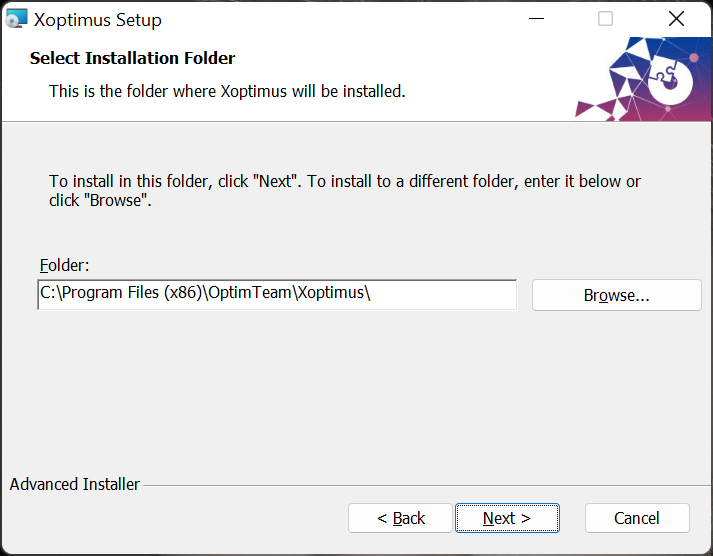
\includegraphics[width=.8\linewidth]{win_2.png}   
	\caption{The user selects the desired installation directory.}   
\label{fig:sfig2} \end{subfigure}
\\
\\
\begin{subfigure}{.55\textwidth}   
\centering   
	
\includegraphics[width=.8\linewidth]{win_3.png}   
	\caption{Prompt to install.}   
\label{fig:sfig3} \end{subfigure}
\begin{subfigure}{.55\textwidth}   
\centering   
	
\includegraphics[width=.8\linewidth]{win_4.png}   
	\caption{Copying files.}   
\label{fig:sfig4} \end{subfigure}
\\
\\
\begin{subfigure}{.55\textwidth}   
\centering   
	
\includegraphics[width=.8\linewidth]{win_5.png}   
	\caption{Finalizing installation.}   
\label{fig:sfig5} \end{subfigure}

\caption{The steps of windows installation\label{fig:windowsInstall}}
\end{figure}

\begin{thebibliography}{100}
\bibitem{globalecon1}Zwe-Lee Gaing, Particle swarm optimization to
solving the economic dispatch considering the generator constraints,
IEEE Transactions on \textbf{18} Power Systems, pp. 1187-1195, 2003.

\bibitem{globalecon2}C. D. Maranas, I. P. Androulakis, C. A. Floudas,
A. J. Berger, J. M. Mulvey, Solving long-term financial planning problems
via global optimization, Journal of Economic Dynamics and Control
\textbf{21}, pp. 1405-1425, 1997.

\bibitem{global_physics1}Q. Duan, S. Sorooshian, V. Gupta, Effective
and efficient global optimization for conceptual rainfall-runoff models,
Water Resources Research \textbf{28}, pp. 1015-1031 , 1992.

\bibitem{global_physics2}P. Charbonneau, Genetic Algorithms in Astronomy
and Astrophysics, Astrophysical Journal Supplement \textbf{101}, p.
309, 1995

\bibitem{global_chemistry1}A. Liwo, J. Lee, D.R. Ripoll, J. Pillardy,
H. A. Scheraga, Protein structure prediction by global optimization
of a potential energy function, Biophysics \textbf{96}, pp. 5482-5485,
1999.

\bibitem{global_chemistry2}P.M. Pardalos, D. Shalloway, G. Xue, Optimization
methods for computing global minima of nonconvex potential energy
functions, Journal of Global Optimization \textbf{4}, pp. 117-133,
1994.

\bibitem{global_med1}Eva K. Lee, Large-Scale Optimization-Based Classification
Models in Medicine and Biology, Annals of Biomedical Engineering \textbf{35},
pp 1095-1109, 2007.

\bibitem{global_med2}Y. Cherruault, Global optimization in biology
and medicine, Mathematical and Computer Modelling \textbf{20}, pp.
119-132, 1994.

\bibitem{global_job1}Y. Gao, H. Rong, J.Z. Huang, Adaptive grid job
scheduling with genetic algorithms, Future Generation Computer Systems
\textbf{21}, pp. 151-161, 2005.

\bibitem{global_job2}D.Y. Sha, H.H. Lin, A multi-objective PESO for
job-shop scheduling problems, Expert Systems with Applications \textbf{37},
pp. 1065-1070, 2010.

\bibitem{global_water1}X. Cai, D.C. McKinney, L.S. Lasdon, Solving
nonlinear water management models using a combined genetic algorithm
and linear programming approach, Advances in Water Resources \textbf{24},
pp. 667-676, 2001.

\bibitem{global_water2}S.G. Gino Sophia, V. Ceronmani Sharmila, S.
Suchitra et al, Water management using genetic algorithm-based machine
learning, Soft Comput \textbf{24}, pp. 17153--17165, 2020.

\bibitem{global_network1}Z. Bankovic, D. Stepanovic, S. Bojanic,
O. Nieto - Taladriz, Improving network security using genetic algorithm
approach, Computers \& Electrical Engineering \textbf{33}, pp. 438-451,
2007.

\bibitem{global_network2}S. Paul, I. Dutt, S.N. Choudhri, Design
and implementation of network security using genetic algorithm. Int
J Res Eng Technol \textbf{2}, pp. 172-177, 2013.

\bibitem{global_robot1}A. Tuncer, M. Yildrim, Dynamic path planning
of mobile robots with improved genetic algorithm, Computers \& Electrical
Engineering \textbf{38}, pp. 1564-1572, 2012.

\bibitem{global_robot2}N. Kherici, Y.M. Ben Ali, Using PESO for a
walk of a biped robot, Journal of Computational Science \textbf{5},
pp. 743-749, 2014.

\bibitem{go_symmetry0}B. Freisleben and P. Merz, A genetic local
search algorithm for solving symmetric and asymmetric traveling salesman
problems, In: Proceedings of IEEE International Conference on Evolutionary
Computation, pp. 616-621, 1996.

\bibitem{go_symmetry1}R. Grbi\'{c}, E.K. Nyarko and R. Scitovski,
A modification of the DIRECT method for Lipschitz global optimization
for a symmetric function, J Glob Optim \textbf{57}, pp. 1193--1212,
2013.

\bibitem{go_symmetry2}R. Scitovski, A new global optimization method
for a symmetric Lipschitz continuous function and the application
to searching for a globally optimal partition of a one-dimensional
set, J Glob Optim \textbf{68}, pp. 713--727, 2017.

\bibitem{global_nonlinear1}Barbara Kaltenbacher and William Rundell,
The inverse problem of reconstructing reaction--diffusion systems,
Invese Problems \textbf{36}, 2020.

\bibitem{global_nonlinear2}N. Levashova, A. Gorbachev, R. Argun,
D. Lukyanenko, The Problem of the Non-Uniqueness of the Solution to
the Inverse Problem of Recovering the Symmetric States of a Bistable
Medium with Data on the Position of an Autowave Front., Symmetry \textbf{13},
2021.

\bibitem{global_nonlinear3}Larisa Beilina, Michael V. Klibanov, A
Globally Convergent Numerical Method for a Coefficient Inverse Problem,
SIAM Journal on Scientific Computing \textbf{31},pp. 478-509, 2008. 

\bibitem{go_adaptive1}M. Brunato, R. Battiti, RASH: A Self-adaptive
Random Search Method. In: Cotta, C., Sevaux, M., S�rensen, K. (eds)
Adaptive and Multilevel Metaheuristics. Studies in Computational Intelligence,
vol 136. Springer, Berlin, Heidelberg, 2008.

\bibitem{go_adaptive2}S. Andrad�ttir, A.A. Prudius, A.A., Adaptive
random search for continuous simulation optimization. Naval Research
Logistics \textbf{57}, pp. 583-604, 2010.

\bibitem{go_crs1}W.L. Price, Global optimization by controlled random
search, J Optim Theory Appl \textbf{40}, pp. 333--348, 1983.

\bibitem{go_crs2}P. Kaelo, M.M. Ali, Some Variants of the Controlled
Random Search Algorithm for Global Optimization. J Optim Theory Appl
\textbf{130}, pp. 253--264 (2006).

\bibitem{go_sa1}S. Kirkpatrick, C.D. Gelatt, M.P. Vecchi, Optimization
by simulated annealing, Science \textbf{220}, pp. 671-680, 1983.

\bibitem{go_sa2}K.M.El-Naggar, M.R. AlRashidi, M.F. AlHajri, A.K.
Al-Othman, Simulated Annealing algorithm for photovoltaic parameters
identification, Solar Energy \textbf{86}, pp. 266-274, 2012.

\bibitem{go_sa3}L.M. Rasdi Rere, M.I. Fanany, A.M. Arymurthy, Simulated
Annealing Algorithm for Deep Learning, Procedia Computer Science \textbf{72},
pp. 137-144, 2015.

\bibitem{go_ga1}J. Mc Call, Genetic algorithms for modelling and
optimisation, Journal of Computational and Applied Mathematics \textbf{184},
pp. 205-222, 2005.

\bibitem{go_ga2}C.K.H. Lee, A review of applications of genetic algorithms
in operations management, Elsevier Engineering Applications of Artificial
Intelligence \textbf{76}, pp. 1-12, 2018.

\bibitem{go_ant1}B. Chandra Mohan, R. Baskaran, A survey: Ant Colony
Optimization based recent research and implementation on several engineering
domain, Expert Systems with Applications \textbf{39}, pp. 4618-4627,
2012.

\bibitem{go_ant2}T. Liao, T. St�tzle, M.A. Montes de Oca, M. Dorigo,
A unified ant colony optimization algorithm for continuous optimization,
European Journal of Operational Research \textbf{234}, pp. 597-609,
2014.

\bibitem{go_pso1}D. Wang, D. Tan, L. Liu, Particle swarm optimization
algorithm: an overview. Soft Comput \textbf{22}, pp. 387--408, 2018.

\bibitem{go_pso2}N.K. Jain, U. Nangia, J. Jain, A Review of Particle
Swarm Optimization. J. Inst. Eng. India Ser. B \textbf{99}, pp. 407--411,
2018.

\bibitem{go_pso_genetic_hybrid1}D.H. Kim, A. Abraham, J.H. Cho, A
hybrid genetic algorithm and bacterial foraging approach for global
optimization, Information Sciences \textbf{177}, pp. 3918-3937, 2007.

\bibitem{go_pso_genetic_hybrid2}Y.T. Kao, E. Zahara, A hybrid genetic
algorithm and particle swarm optimization for multimodal functions,
Applied Soft Computing \textbf{8}, pp. 849-857, 2008.

\bibitem{ga_fuzzy}G.T. Reddy, M.P.K. Reddy, K. Lakshmanna et al,
Hybrid genetic algorithm and a fuzzy logic classifier for heart disease
diagnosis, Evol. Intel. \textbf{13}, pp. 185--196, 2020.

\bibitem{ga_kmeans}M.D. Anisur Rahman, M.D. Zahidul Islam, A hybrid
clustering technique combining a novel genetic algorithm with K-Means,
Knowledge-Based Systems \textbf{71}, pp. 345-365, 2014.

\bibitem{pso_aco1}T. Niknam, An efficient hybrid evolutionary algorithm
based on PESO and ACO for distribution feeder reconfiguration, European
Transactions on Electrical Power \textbf{20}, pp. 575-590, 2010.

\bibitem{pso_aco2}M.K. Patel, M.R. Kabat, C.R. Tripathy, A hybrid
ACO/PESO based algorithm for QoS multicast routing problem, Ain Shams
Engineering Journal \textbf{5}, pp. 113-120, 2014.

\bibitem{pso_aco3}A.K. Dubey, A. Kumar, R. Agrawal, An efficient
ACO-PSO-based framework for data classification and preprocessing
in big data, Evol. Intel. \textbf{14}, pp. 909--922, 2021.

\bibitem{hybrid1}Offord C., Bajzer �. (2001) A Hybrid Global Optimization
Algorithm Involving Simplex and Inductive Search. In: Alexandrov V.N.,
Dongarra J.J., Juliano B.A., Renner R.S., Tan C.J.K. (eds) Computational
Science - ICCS 2001. ICCS 2001. Lecture Notes in Computer Science,
vol 2074. Springer, Berlin, Heidelberg.

\bibitem{go_local1}S. Li, M. Tan, I. W. Tsang, J. T. -Y. Kwok, A
Hybrid PSO-BFGS Strategy for Global Optimization of Multimodal Functions,
IEEE Transactions on Systems, Man, and Cybernetics, Part B (Cybernetics)
\textbf{41}, pp. 1003-1014, 2011.

\bibitem{go_local2}H. Badem, A. Basturk, A. Caliskan, M.E. Yuksel,
A new hybrid optimization method combining artificial bee colony and
limited-memory BFGS algorithms for efficient numerical optimization,
Applied Soft Computing \textbf{70}, pp. 826-844, 2018.

\bibitem{go_local3}A.A. Nagra, F. Han, Q.H. Ling, An improved hybrid
self-inertia weight adaptive particle swarm optimization algorithm
with local search, Engineering Optimization \textbf{51}, pp. 1115-1132,
2018.

\bibitem{genetic_physics1}S.Q. Wu, M. Ji, C.Z. Wang, M.C. Nguyen,
X. Zhao, K. Umemoto, R. M. Wentzcovitch, K. M. Ho, An adaptive genetic
algorithm for crystal structure prediction, Journal of Physics: Condensed
Matter \textbf{26}, 035402, 2013.

\bibitem{genetic_physics2}M. Honda, Application of genetic algorithms
to modelings of fusion plasma physics, Computer Physics Communications
\textbf{231}, pp. 94-106, 2018.

\bibitem{genetic_physics3}X.L. Luo, J. Feng, H.H. Zhang, A genetic
algorithm for astroparticle physics studies, Computer Physics Communications
\textbf{250}, 106818, 2020.

\bibitem{pso_physics1}M. Ye, X. Wang, Y. Xu, Parameter extraction
of solar cells using particle swarm optimization, Journal of Applied
Physics \textbf{105}, 094502. 2009.

\bibitem{pso_physics2}A. Belkadi, L. Ciarletta, D. Theilliol, Particle
swarm optimization method for the control of a fleet of Unmanned Aerial
Vehicles, Journal of Physics: Conference Series, Volume 659, 12th
European Workshop on Advanced Control and Diagnosis (ACD 2015) 19--20
November 2015, Pilsen, Czech Republic.

\bibitem{async1}M. Depolli, R. Trobec, B. Filipi\v{c}, Asynchronous
Master-Slave Parallelization of Differential Evolution for Multi-Objective
Optimization, Evolutionary Computation \textbf{21}, pp. 261-291, 2013.

\bibitem{async2}A. P. Engelbrecht, Asynchronous particle swarm optimization
with discrete crossover, In: 2014 IEEE Symposium on Swarm Intelligence,
Orlando, FL, USA, 2014, pp. 1-8.

\bibitem{async3}F. Bourennani, Cooperative asynchronous parallel
particle swarm optimization for large dimensional problems, International
Journal of Applied Metaheuristic Computing (IJAMC) \textbf{10.3},
pp. 19-38, 2019.

\bibitem{parallel-multistart}J. Larson and S.M. Wild, Asynchronously
parallel optimization solver for finding multiple minima, Mathematical
Programming Computation \textbf{10}, pp. 303-332, 2018.

\bibitem{parallel-multistart2}H.P.J. Bolton, J.F. Schutte, A.A. Groenwold,
Multiple Parallel Local Searches in Global Optimization. In: Dongarra
J., Kacsuk P., Podhorszki N. (eds) Recent Advances in Parallel Virtual
Machine and Message Passing Interface. EuroPVM/MPI 2000. Lecture Notes
in Computer Science, vol 1908. Springer, Berlin, Heidelberg, 2000.

\bibitem{gpu1}Y. Zhou and Y. Tan, GPU-based parallel particle swarm
optimization, In: 2009 IEEE Congress on Evolutionary Computation,
2009, pp. 1493-1500.

\bibitem{gpu2}L. Dawson and I. Stewart, Improving Ant Colony Optimization
performance on the GPU using CUDA, In: 2013 IEEE Congress on Evolutionary
Computation, 2013, pp. 1901-1908.

\bibitem{gpu3}Barkalov, K., Gergel, V. Parallel global optimization
on GPU. J Glob Optim \textbf{66}, pp. 3--20, 2016.

\bibitem{baron}N.V. Sahinidis, BARON: A general purpose global optimization
software package, J Glob Optim \textbf{8}, pp. 201--205, 1996.

\bibitem{merlin}D.G. Papageorgiou, I.N. Demetropoulos, I.E. Lagaris,
Computer Physics Communications \textbf{159}, pp. 70-71, 2004.

\bibitem{deoptim}K. Mullen, D. Ardia, D.L. Gil, D. Windover, J. Cline,
DEoptim: An R Package for Global Optimization by Differential Evolution,
Journal of Statistical Software \textbf{40}, pp. 1-26, 2011.

\bibitem{pdoublepop}I.G. Tsoulos, A. Tzallas, D. Tsalikakis, PDoublePop:
An implementation of parallel genetic algorithm for function optimization,
Computer Physics Communications \textbf{209}, pp. 183-189, 2016.

\bibitem{paradiseo}J. Dreo, A. Liefooghe, S. Verel, M. Schoenauer,
J.J. Merelo, A. Quemy, B. Bouvier, J. Gmys, Paradiseo: from a modular
framework for evolutionary computation to the automated design of
metaheuristics ---22 years of Paradiseo---, GECCO'21: Proceedings
of the Genetic and Evolutionary Computation Conference Companion,
1522--1530, 2021.

\bibitem{pagmo}F. Biscani, D. Izzo, A parallel global multiobjective
framework for optimization: pagmo, Journal of Open Source Software
\textbf{5}, 2338, 2020.

\bibitem{de_main_paper}R. Storn, On the usage of differential evolution
for function optimization, In: Proceedings of North American Fuzzy
Information Processing, pp. 519-523, 1996.

\bibitem{de_datamining}I. Triguero, S. Garcia, F. Herrera, Differential
evolution for optimizing the positioning of prototypes in nearest
neighbor classification, Pattern Recognition \textbf{44}, pp. 901-916,
2011.

\bibitem{de_symmetry1}Y.H. Li, J.Q. Wang, X.J. Wang, Y.L. Zhao, X.H.
Lu, D.L. Liu, Community Detection Based on Differential Evolution
Using Social Spider Optimization, Symmetry \textbf{9}, 2017.

\bibitem{de_symmetry3}W. Yang, E.M. Dilanga Siriwardane, R. Dong,
Y. Li, J. Hu, Crystal structure prediction of materials with high
symmetry using differential evolution, J. Phys.: Condens. Matter \textbf{33}
455902, 2021.

\bibitem{de_symmetry6}C.Y. Lee, C.H. Hung, Feature Ranking and Differential
Evolution for Feature Selection in Brushless DC Motor Fault Diagnosis
, Symmetry \textbf{13}, 2021.

\bibitem{de_symmetry7}S. Saha, R. Das, Exploring differential evolution
and particle swarm optimization to develop some symmetry-based automatic
clustering techniques: application to gene clustering, Neural Comput
\& Applic \textbf{30}, pp. 735--757, 2018.

\bibitem{parallelDe}V. Charilogis, I.G. Tsoulos, A Parallel Implementation
of the Differential Evolution Method, Analytics \textbf{2}, pp. 17-30,
2023.

\bibitem{openMp}R. Chandra, L. Dagum, D. Kohr, D. Maydan,J. McDonald
and R. Menon, Parallel Programming in OpenMP, Morgan Kaufmann Publishers
Inc., 2001.

\bibitem{doublepop_tsoulos}I.G. Tsoulos, Modifications of real code
genetic algorithm for global optimization, Applied Mathematics and
Computation \textbf{203}, pp. 598-607, 2008.

\bibitem{genetic1}J.F.Gon�alves, J.J.M. Mendes, M.G.C. Resende, A
genetic algorithm for the resource constrained multi-project scheduling
problem, European Journal of Operational Research \textbf{189}, pp.
1171-1190, 2008.

\bibitem{genetic2}W.Ho, G.T.S. Ho, P. Ji, H.C.W. Lau, A hybrid genetic
algorithm for the multi-depot vehicle routing problem, Engineering
Applications of Artificial Intelligence \textbf{21}, pp. 548-557,
2008.

\bibitem{genetic3}J.F. Gon�alves, M.G.C. Resende, Biased random-key
genetic algorithms for combinatorial optimization. J Heuristics \textbf{17},
pp. 487--525, 2011.

\bibitem{genetic4}M. Turrin, P. Buelow, R. Stouffs, Design explorations
of performance driven geometry in architectural design using parametric
modeling and genetic algorithms, Advanced Engineering Informatics
\textbf{25}, pp. 656-675, 2011.

\bibitem{psoApp1}M. Ye, X. Wang, Y. Xu, Parameter extraction of solar
cells using particle swarm optimization, Journal of Applied Physics
\textbf{105}, 094502, 2009.

\bibitem{psoApp2}Y. Wang, J. Lv, L. Zhu, Y. Ma, Crystal structure
prediction via particle-swarm optimization, Phys. Rev. B \textbf{82},
094116, 2010.

\bibitem{psoApp3}M. Weiel, M. G�tz, A. Klein et al, Dynamic particle
swarm optimization of biomolecular simulation parameters with flexible
objective functions. Nat Mach Intell \textbf{3}, pp. 727--734, 2021.

\bibitem{ipso}V. Charilogis, I.G. Tsoulos, Toward an Ideal Particle
Swarm Optimizer for Multidimensional Functions, Information \textbf{13},
217, 2022.

\bibitem{multistart-tsp}Li W., A Parallel Multi-start Search Algorithm
for Dynamic Traveling Salesman Problem. In: Pardalos P.M., Rebennack
S. (eds) Experimental Algorithms. SEA 2011. Lecture Notes in Computer
Science, vol 6630. Springer, Berlin, Heidelberg, 2011.

\bibitem{multistart-vehicle}Olli Br�ysy, Geir Hasle, Wout Dullaert,
A multi-start local search algorithm for the vehicle routing problem
with time windows, European Journal of Operational Research \textbf{159},
pp. 586-605, 2004.

\bibitem{multistart_fac}Mauricio G.C. Resende, Renato F. Werneck,A
hybrid multistart heuristic for the uncapacitated facility location
problem, European Journal of Operational Research \textbf{174}, pp.
54-68, 2006.

\bibitem{multistart_clique}E. Marchiori, Genetic, Iterated and Multistart
Local Search for the Maximum Clique Problem. In: Cagnoni S., Gottlieb
J., Hart E., Middendorf M., Raidl G.R. (eds) Applications of Evolutionary
Computing. EvoWorkshops 2002. Lecture Notes in Computer Science, vol
2279. Springer, Berlin, Heidelberg. 

\bibitem{multistart_fire}Gomes M.I., Afonso L.B., Chibeles-Martins
N., Fradinho J.M. (2018) Multi-start Local Search Procedure for the
Maximum Fire Risk Insured Capital Problem. In: Lee J., Rinaldi G.,
Mahjoub A. (eds) Combinatorial Optimization. ISCO 2018. Lecture Notes
in Computer Science, vol 10856. Springer, Cham. https://doi.org/10.1007/978-3-319-96151-4\_19

\bibitem{multistart-aero}Streuber, Gregg M. and Zingg, David. W.,
Evaluating the Risk of Local Optima in Aerodynamic Shape Optimization,
AIAA Journal 59, pp. 75-87, 2012.

\bibitem{rbf_main1}J. Park, I.W. Sandberg, Approximation and Radial-Basis-Function
Networks, Neural Computation \textbf{5}, pp. 305-316, 1993.

\bibitem{neuralMinimizer}I.G. Tsoulos, A. Tzallas, E. Karvounis,
D. Tsalikakis, NeuralMinimizer, a novel method for global optimization
that incorporates machine learning, Information \textbf{14}, 2, 2023.

\bibitem{ppso}V. Charilogis, I.G. Tsoulos, A. Tzallas, An Improved
Parallel Particle Swarm Optimization, SN COMPUT. SCI. \textbf{4},
766, 2023.

\bibitem{corana}A. Corana, M. Marchesi, C. Martini, S. Ridella, Minimizing
multimodal functions of continuous variables with the \textquotedblleft Simulated
Annealing\textquotedblright{} algo- rithm, ACM Trans. Math. Software
\textbf{13}, pp. 262--280, 1987.

\bibitem{ofa1}Kyrou, G., Charilogis, V., \& Tsoulos, I. G. (2024).
EOFA: An Extended Version of the Optimal Foraging Algorithm for Global
Optimization Problems. Computation, 12(8), 158.

\bibitem{ofa2}Ding, C., \& Zhu, G. (2024). Improved optimal foraging
algorithm for global optimization. Computing, 1-27.

\bibitem{gao1}Kyrou, G., Charilogis, V., \& Tsoulos, I. G. (2024).
Improving the Giant-Armadillo Optimization Method. Analytics, 3(2),
225-240.

\bibitem{gao2}Alsayyed, O., Hamadneh, T., Al-Tarawneh, H., Alqudah,
M., Gochhait, S., Leonova, I., ... \& Dehghani, M. (2023). Giant Armadillo
optimization: A new bio-inspired metaheuristic algorithm for solving
optimization problems. Biomimetics, 8(8), 619.

\bibitem{gwo}Mirjalili, S., Mirjalili, S. M., \& Lewis, A. (2014).
Grey wolf optimizer. Advances in engineering software, 69, 46-61.

\bibitem{powell}M.J.D Powell, A Tolerant Algorithm for Linearly Constrained
Optimization Calculations, Mathematical Programming \textbf{45}, pp.
547-566, 1989. 

\bibitem{lbfgs}D.C. Liu, J. Nocedal, On the Limited Memory Method
for Large Scale Optimization, Mathematical Programming B \textbf{45},
pp. 503-528, 1989.

\bibitem{gradient1}S.I. Amari, Backpropagation and stochastic gradient
descent method, Neurocomputing \textbf{5}, pp. 185-196, 1993.

\bibitem{gradient2}S. Klein, J.P.W. Pluim, M. Staring, Adaptive Stochastic
Gradient Descent Optimisation for Image Registration, Int J Comput
Vis \textbf{81}, pp. 227--239, 2009.

\bibitem{nelderMead}D.M. Olsson,L.S. Nelson, The Nelder-Mead Simplex
Procedure for Function Minimization, Technometrics \textbf{17}, pp.
45-51, 1975.

\bibitem{Adam}D.P. Kingma, J. Ba, Adam: A Method for Stochastic Optimization,
ICLR (Poster), 2015.

\bibitem{adept}R.J. Hogan, Fast reverse-mode automatic differentiation
using expression templates in C++. ACM Trans. Math. Softw. \textbf{40},
pp. 1-26, 2014.

\bibitem{originalJones}J.E. Lennard-Jones, On the Determination of
Molecular Fields, Proc. R. Soc. Lond. A \textbf{ 106}, pp. 463--477,
1924.

\bibitem{nn1}C. Bishop, Neural Networks for Pattern Recognition,
Oxford University Press, 1995.

\bibitem{nn2}G. Cybenko, Approximation by superpositions of a sigmoidal
function, Mathematics of Control Signals and Systems \textbf{2}, pp.
303-314, 1989.

\bibitem{testfunctions1}M.M. Ali and P. Kaelo, Improved particle
swarm algorithms for global optimization, Applied Mathematics and
Computation \textbf{196}, pp. 578-593, 2008.

\bibitem{testfunctions2}H. Koyuncu, R. Ceylan, A PESO based approach:
Scout particle swarm algorithm for continuous global optimization
problems, Journal of Computational Design and Engineering \textbf{6},
pp. 129--142, 2019.

\bibitem{testfunctions3}Patrick Siarry, G�rard Berthiau, Fran�ois
Durdin, Jacques Haussy, ACM Transactions on Mathematical Software
\textbf{23}, pp 209--228, 1997.

\bibitem{testfunctions4}I.G. Tsoulos, I.E. Lagaris, GenMin: An enhanced
genetic algorithm for global optimization, Computer Physics Communications\textbf{
178, }pp. 843-851, 2008.

\bibitem{Jones}J.A. Northby, Structure and binding of Lennard-Jones
clusters: 13 \ensuremath{\le} n \ensuremath{\le} 147, J. Chem. Phys.
\textbf{87}, pp. 6166--6178, 1987.

\bibitem{fuchss} B. K. Ridley, Electrons and Phonons in Semiconductor
Multilayers, Cambridge University Press, 2nd edition (2014) 

\bibitem{jonesNew}G.L. Xue, R.S. Maier, J.B. Rosen, Improvements
on the Northby Algorithm for molecular conformation: Better solutions,
J. Global. Optim. 4, pp. 425--440, 1994.

\bibitem{triangular}W.E. Stein, M.F. Keblis, A new method to simulate
the triangular distribution, Mathematical and Computer Modelling Volume
\textbf{49}, pp. 1143-1147, 2009.

\bibitem{kmeansNew}M. Ahmed, R. Seraj, S.M.S. Islam, The k-means
algorithm: A comprehensive survey and performance evaluation, Electronics
\textbf{9}, 1295, 2020.

\end{thebibliography}

\end{document}
